\documentclass{standalone}
\usepackage{tikz}
\usetikzlibrary{arrows.meta, positioning, shapes}
\usepackage{xcolor}

\definecolor{CentralBlue}{RGB}{0,84,103}
\definecolor{InfographicBG}{RGB}{19,34,52}
\pagestyle{empty}

\pagecolor{InfographicBG}
\begin{document}

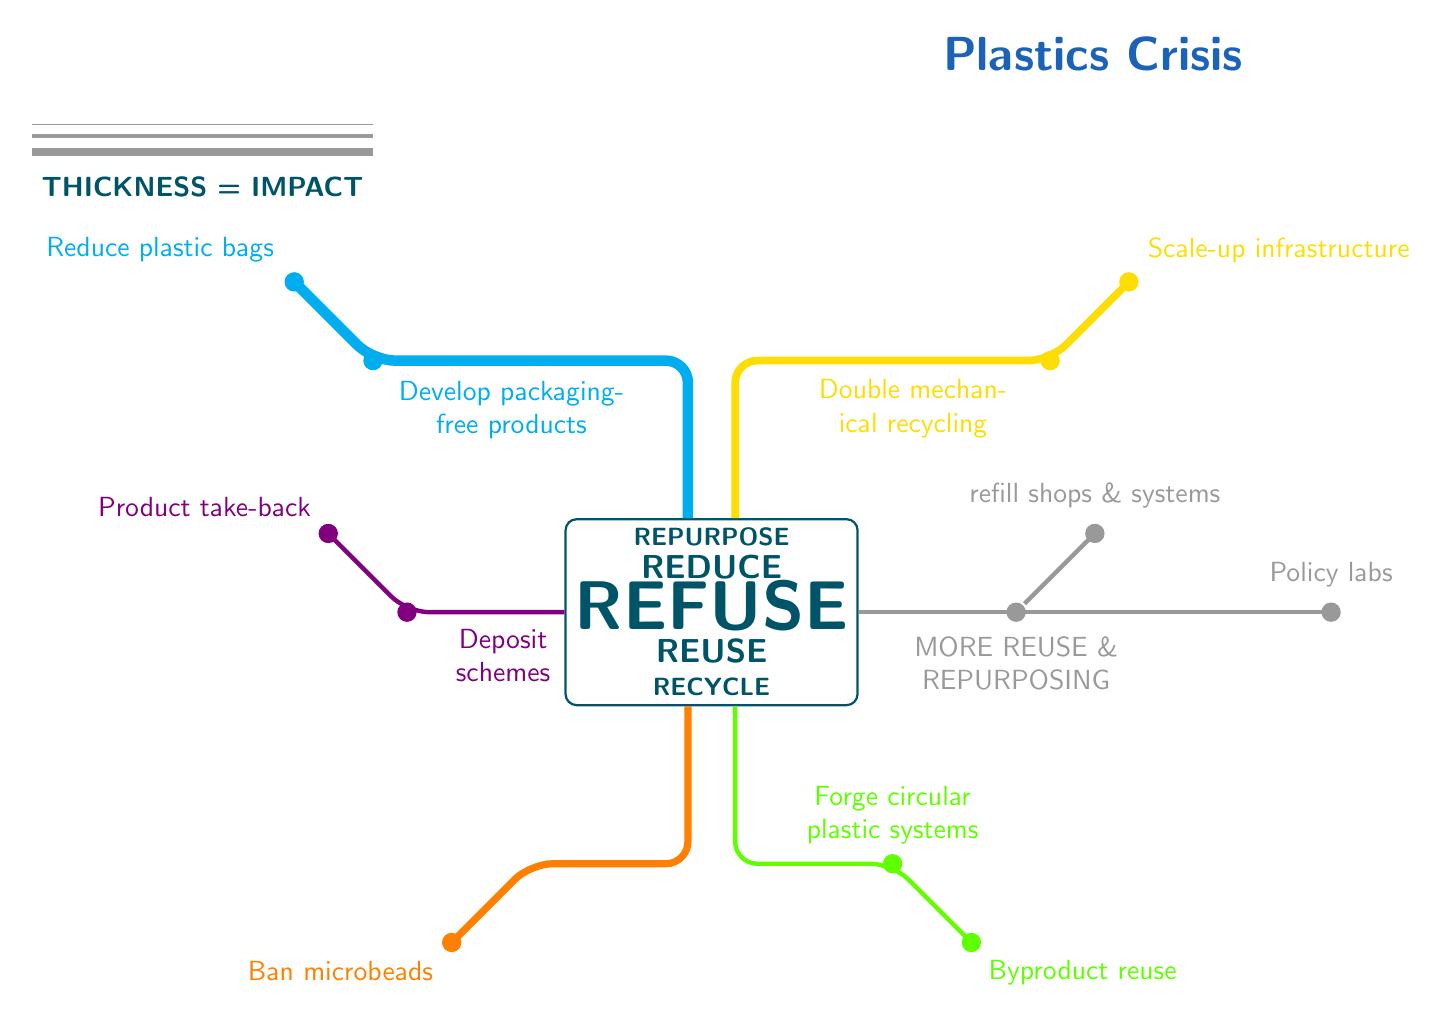
\begin{tikzpicture}[
  font=\sffamily,
  every node/.style={align=center},
  dot/.style={circle, fill=#1, minimum size=7pt, inner sep=0pt},
  route/.style args={#1, #2}{rounded corners=8pt, line width=#1, draw=#2}
  ]

% Central node
\node[draw=CentralBlue, thick, rounded corners, text=CentralBlue] (core) at (0,0) {
  \textbf{\small REPURPOSE}\\
  \textbf{\large REDUCE}\\
  \textbf{\Huge REFUSE}\\
  \textbf{\large REUSE}\\
  \textbf{\small RECYCLE}
  };
 
% Blue: Reduce Plastic Production
\draw[route={3.8pt, cyan}] ([xshift=-0.3cm]core.north) |- ++(-4,2)
  node[dot=cyan] {} node[text width=3cm, below right=3pt, text=cyan] {Develop packaging-free products}
  -- ++(-1,1) node[dot=cyan] {} node[above left=3pt, text=cyan] (label) {Reduce plastic bags};

% Yellow: Better & Increased Recycling
\draw[route={2.8pt, yellow!80!orange}] ([xshift=0.3cm]core.north) |- ++(4,2) node[dot=yellow!80!orange] {} node[text width=3cm, below left=3pt, text=yellow!80!orange] {Double mechanical recycling}
  -- ++(1,1) node[dot=yellow!80!orange] {} node[above right=3pt, text=yellow!80!orange] {Scale-up infrastructure};

% Green: Thinking Circular
\draw[route={1.6pt, lime!50!green}] ([xshift=0.3cm]core.south) |- ++(2,-2)
  node[dot=lime!50!green] {} node[text width=3cm, above=3pt, text=lime!50!green] {Forge circular plastic systems}
  -- ++(1,-1) node[dot=lime!50!green] {} node[below right=3pt, text=lime!50!green] {Byproduct reuse};

% Orange: Extend Bans
\draw[route={2.6pt, orange}] ([xshift=-0.3cm]core.south) |- ++(-2,-2)
  -- ++(-1,-1)
  node[dot=orange] {} node[below left=3pt, text=orange] {Ban microbeads};

% Purple: Clean-ups & Takebacks
\draw[route={1.6pt, violet}] (core.west) -- ++(-2,0)
  node[dot=violet] {} node[text width=2cm, below right=3pt, text=violet] {Deposit schemes}
  -- ++(-1,1) node[dot=violet] {} node[above left=3pt, text=violet] {Product take-back};
 
%Right side branch with split
\draw[route={1.6pt, gray!80}] (core.east) -- ++(2,0)
  node[dot=gray!80](point) {} node[text width=3cm, below=5pt, text=gray!80] {MORE REUSE \&
REPURPOSING} -- ++(4,0)
  node[dot=gray!80] {} node[above=5pt, text=gray!80] {Policy labs};
\draw[route={1.6pt, gray!80}] (point) -- ++(1,1)
  node[dot=gray!80] {} node[above=5pt, text=gray!80] {refill shops \& systems};
  
 % Legend (Top Left)
\node[anchor=south west, text=CentralBlue] at ([yshift=0.2cm]label.north west) (legend) {\textbf{THICKNESS = IMPACT}};
\draw[line width=3pt, gray!80] ([yshift=0.2cm]legend.north west) -- ([yshift=0.2cm]legend.north east);
\draw[line width=1.5pt, gray!80] ([yshift=0.4cm]legend.north west) -- ([yshift=0.4cm]legend.north east);
\draw[line width=0.5pt, gray!80] ([yshift=0.55cm]legend.north west) -- ([yshift=0.55cm]legend.north east);

% Title
\node[anchor=south west, text=white] at ([xshift=-0.6cm, yshift=1cm]legend.north east) {
  \fontsize{16}{18}\selectfont\textbf{Our Routes for Solving the \textcolor{cyan!40!blue}{Plastics Crisis}}
};
\end{tikzpicture}

\end{document}
